% Created 2022-02-19 Sat 13:36
% Intended LaTeX compiler: pdflatex
\documentclass[11pt]{article}
\usepackage[utf8]{inputenc}
\usepackage[T1]{fontenc}
\usepackage{graphicx}
\usepackage{longtable}
\usepackage{wrapfig}
\usepackage{rotating}
\usepackage[normalem]{ulem}
\usepackage{amsmath}
\usepackage{amssymb}
\usepackage{capt-of}
\usepackage{hyperref}
\author{Adam Smith}
\date{\today}
\title{Thesis title}
\hypersetup{
 pdfauthor={Adam Smith},
 pdftitle={Thesis title},
 pdfkeywords={},
 pdfsubject={},
 pdfcreator={Emacs 27.2 (Org mode 9.6)}, 
 pdflang={English}}
\begin{document}

\maketitle
\begin{abstract}
In this thesis we show that \ldots{}
\end{abstract}



\newpage



\setcounter{tocdepth}{2}
\tableofcontents


\section{Introduction}
\label{sec:org566bd8f}
\label{sec:intro}



\section{Literature references}
\label{sec:org729d046}


\subsection{org cite}
\label{sec:org88254cd}

\url{https://blog.tecosaur.com/tmio/2021-07-31-citations.html}

(Athey, Susan and Imbens, Guido W., 2019)



\subsection{org-ref}
\label{sec:org25e86c2}


\url{https://github.com/jkitchin/org-ref}

See \cite{armstrong-2007-chapt-coord} for an analysis. We can also have references between brackets \citep{athey-2019-machin-learn}.


\section{Model}
\label{sec:org84e90fc}

As we explained in section \ref{sec:intro}.

Here we have some in-line math: \(x^2\).\footnote{This is a footnote.}

\begin{equation}
\label{eq:1}
a^2 + b^2 = c^2
\end{equation}

As we show in equation \eqref{eq:1}.

\begin{table}[htbp]
\caption{\label{table1}This table shows unemployment and gdp per head.}
\centering
\begin{tabular}{lrr}
country & unemployment & gdp\\
\hline
NL & 0.06 & 20000\\
UK & 0.01 & 19500\\
BE & 0.08 & 21100\\
\hline
average & 0.05 & 20200\\
\end{tabular}
\end{table}


\begin{verbatim}
import numpy as np
import pandas as pd
X = np.array(data)
plt.plot(X[1:,2],X[1:,1],'o')
plt.savefig('./fig.png')
\end{verbatim}

\begin{verbatim}
/tmp/babel-URrt4d/python-daaqjg
\end{verbatim}


\begin{verbatim}
df = pd.DataFrame(X[1:,:],columns=X[0,:])
df
\end{verbatim}

\begin{verbatim}
   country unemployment    gdp
0       NL         0.06  20000
1       UK         0.01  19500
2       BE         0.08  21100
3  average         0.05  20200
\end{verbatim}


\begin{verbatim}
import matplotlib.pyplot as plt
plt.plot(df.gdp,df.unemployment,'o')
plt.savefig('./fig.png')
\end{verbatim}

\begin{verbatim}
None
\end{verbatim}


\begin{figure}[htbp]
\centering
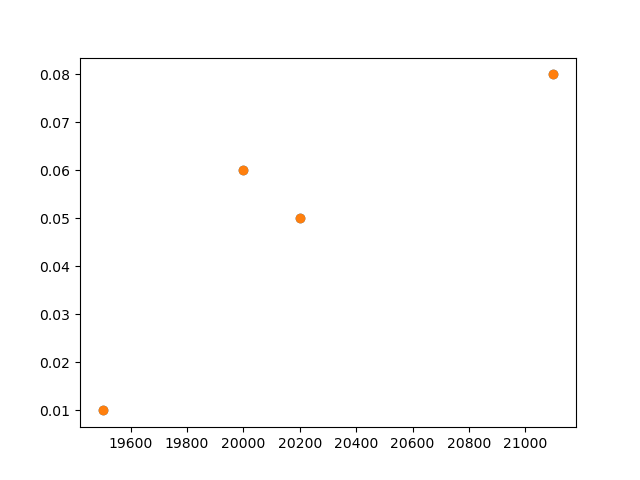
\includegraphics[width=.9\linewidth]{./fig.png}
\caption{\label{figure1}Figure with unemployment and gdp}
\end{figure}

See Figure \ref{figure1}.

\section{Conclusion}
\label{sec:org05aefe3}



\section{Bibliography}
\label{sec:org0df9e45}

\subsection{org ref}
\label{sec:org81dd431}

\bibliography{references}

\subsection{org cite}
\label{sec:orgd3c1741}

\noindent
Athey, Susan and Imbens, Guido W. (2019). \emph{Machine Learning Methods That Economists Should Know About}, Annual Review of Economics.
\end{document}
